%%%%%%%%%%%%%%%%%%%%%%%%%%%%%%%%%%%%%%%%%
% Eleições 2014 - Notícias dos Candidatos
% Apresentação do Analisador Léxico
%
% Lennon Alves
% Felipe Gusmão
%%%%%%%%%%%%%%%%%%%%%%%%%%%%%%%%%%%%%%%%%

\usepackage[utf8]{inputenc}

%----------------------------------------------------------------------------------------
%	Slide 1 - Título
%----------------------------------------------------------------------------------------

\title[Atividade Extra 02]{Eleições 2014 - Análise das Notícias dos Candidatos}

\author{Lennon Alves \\ Felipe Gusmão}
\institute[UTFPR]
{
Universidade Tecnológica Federal do Paraná \\ 
\medskip
\textit{Compiladores}
}
\date{16 Outubro, 2014}

\begin{document}

\begin{frame}
\titlepage
\end{frame}


%----------------------------------------------------------------------------------------
%	Slide 2 - Sumário
%----------------------------------------------------------------------------------------

\begin{frame}
\frametitle{Sumário}
\tableofcontents

\section{Descrição}
\subsection{Cenário (Eleições 2014)}
\subsection{Conjunto de Textos}
\subsection{Proposta e Objetivo}
\section{Análise Léxica}
\section{Análise dos Resultados}

\end{frame}

%----------------------------------------------------------------------------------------
%	Slide 3 - Descrição
%----------------------------------------------------------------------------------------

\begin{frame}
\frametitle{Eleições Gerais Brasileiras}
As eleições de 2014 foram realizadas no dia 05 de outubro, onde elegeu governadores, senadores e deputados.
\\~\\
Esse ano, teremos mais uma eleição decidida em segundo turno para a presidência do Brasil, a mesma irá ocorrer entre o candidato de oposição Aécio Neves e a atual presidenta, Dilma Rousseff.
\end{frame}

%----------------------------------------------------------------------------------------
%	Slide 4 - Descrição
%----------------------------------------------------------------------------------------

\begin{frame}
\frametitle{Conjunto de Textos}
Os textos foram retirados de alguns dos portais de notícias mais acessados na internet, em páginas cujo foco seja política no Brasil. Essas páginas, seja html ou xml (feeds), foram introduzidas ao analisador para efetuar as regras descritas nos próximos slides.
\end{frame}

%----------------------------------------------------------------------------------------
%	Slide 5 - Descrição
%----------------------------------------------------------------------------------------

\begin{frame}
\frametitle{Proposta e Objetivo}
\begin{block}{Proposta}
Com a aproximação do segundo turno das eleições e o clima entre os candidatos cada vez mais tenso, nós buscamos através de sites e feeds, notícias envolvendo o nome do candidato Aécio Neves e da candidata Dilma Rousseff.
\end{block}

\begin{block}{Objetivo}
O objetivo é, através de uma análise léxica sobre o conteúdo obtido através das informações obtidas, verificar a presência ou ausència da cada candidato, entre os portais de notícias escolhido. Analisamos também palavras chave, como "saúde", "educação" e "segurança", buscando as importâncias desses dados e conferindo a parcialidade de cada central de notícias.
\end{block}
\end{frame}

%----------------------------------------------------------------------------------------
%	Slide 6 - Análise Léxica
%----------------------------------------------------------------------------------------

\begin{frame}[fragile]
\frametitle{Análise Léxica}
\begin{example}[Palavras Chave]
\begin{verbatim}
SAUDE						sa(u|ú)de
EDUCACAO					educa(c|ç)(a|ã)o
SEGURANCA					seguran(c|ç)a\end{verbatim}
\end{example}
\end{frame}

%----------------------------------------------------------------------------------------
%	Slide 7 - Análise Léxica
%----------------------------------------------------------------------------------------

\begin{frame}[fragile]
\frametitle{Análise Léxica}
\begin{example}[Busca candidato Aécio]
\begin{verbatim}
BUSCAAECIO 					a(e|é)cio
SAUDEAECIO 					({SAUDE}.*{BUSCAAECIO})
|({BUSCAAECIO}.*{SAUDE})
EDUCACAOAECIO				({EDUCACAO}.*{BUSCAAECIO})
|({BUSCAAECIO}.*{EDUCACAO})
SEGURANCAAECIO				({SEGURANCA}.*{BUSCAAECIO})
|({BUSCAAECIO}.*{SEGURANCA})

SAUDEEDUCACAOAECIO			({SAUDEAECIO}{EDUCACAOAECIO})
|({EDUCACAOAECIO}{SAUDEAECIO})
SAUDESEGURANCAAECIO			({SAUDEAECIO}{SEGURANCAAECIO})
|({SEGURANCAAECIO}|{SAUDEAECIO})
EDUCACAOSEGURANCAAECIO		({EDUCACAOAECIO}{SEGURANCAAECIO})
|({SEGURANCAAECIO}|{EDUCACAOAECIO})\end{verbatim}
\end{example}
\end{frame}

%----------------------------------------------------------------------------------------
%	Slide 8 - Análise Léxica
%----------------------------------------------------------------------------------------

\begin{frame}[fragile]
\frametitle{Análise Léxica}
\begin{example}[Busca candidata Dilma]
\begin{verbatim}
BUSCADILMA 					dilma
SAUDEDILMA 					({SAUDE}.*{BUSCADILMA})
|({BUSCADILMA}.*{SAUDE})
EDUCACAODILMA				({EDUCACAO}.*{BUSCADILMA})
|({BUSCADILMA}.*{EDUCACAO})
SEGURANCADILMA				({SEGURANCA}.*{BUSCADILMA})
|({BUSCADILMA}.*{SEGURANCA})

SAUDEEDUCACAODILMA			({SAUDEDILMA}{EDUCACAODILMA})
|({EDUCACAODILMA}{SAUDEDILMA})
SAUDESEGURANCADILMA			({SAUDEDILMA}{SEGURANCADILMA})
|({SEGURANCADILMA}{SAUDEDILMA})
EDUCACAOSEGURANCADILMA		({EDUCACAODILMA}{SEGURANCADILMA})
|({SEGURANCADILMA}{EDUCACAODILMA})\end{verbatim}
\end{example}
\end{frame}

%----------------------------------------------------------------------------------------
%	Slide 9 - Análise dos Resultados
%----------------------------------------------------------------------------------------

\begin{frame}[fragile]
\frametitle{Análise dos Resultados}
\begin{figure} 
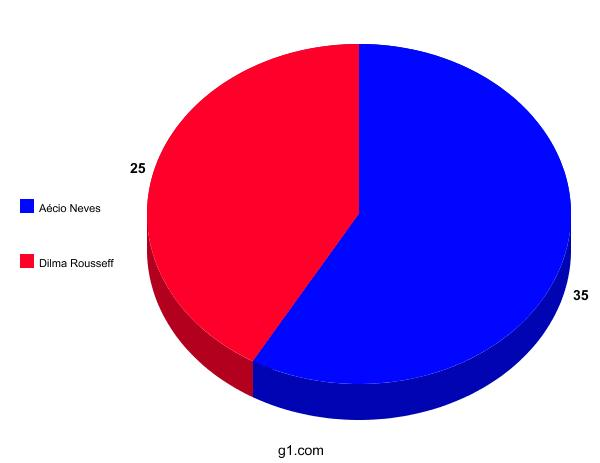
\includegraphics[width=0.4\paperheight]{graph-g1.jpg}
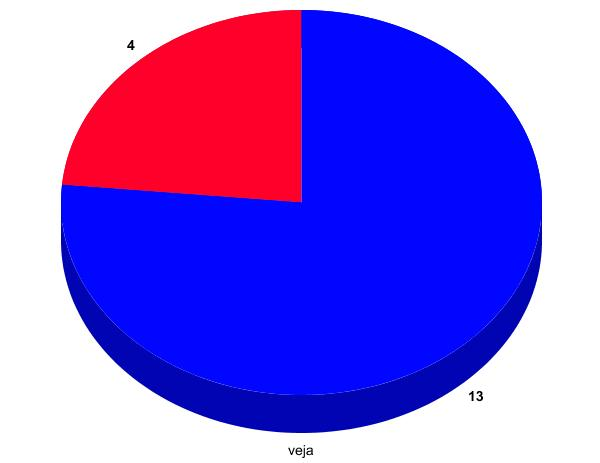
\includegraphics[width=0.4\paperheight]{graph-veja.jpg}
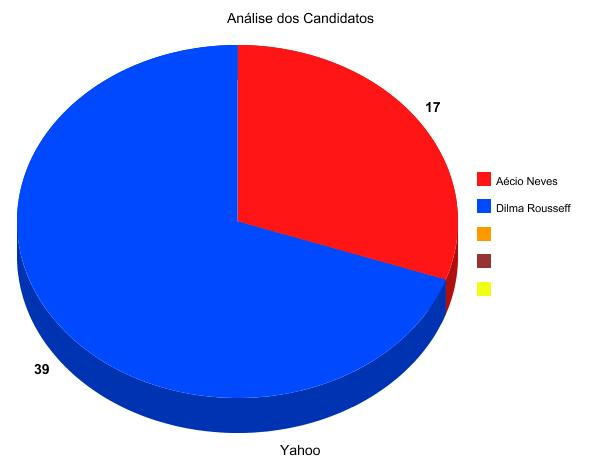
\includegraphics[width=0.4\paperheight]{graph-yahoo.jpg}
\caption{Comparação da quantidade de notícias envolvendo "Aécio" e "Dilma".}
\end{figure}
\end{frame}

%----------------------------------------------------------------------------------------
%	Slide 10 - Análise dos Resultados
%----------------------------------------------------------------------------------------

\begin{frame}[fragile]
\frametitle{Análise dos Resultados}
\begin{figure} 
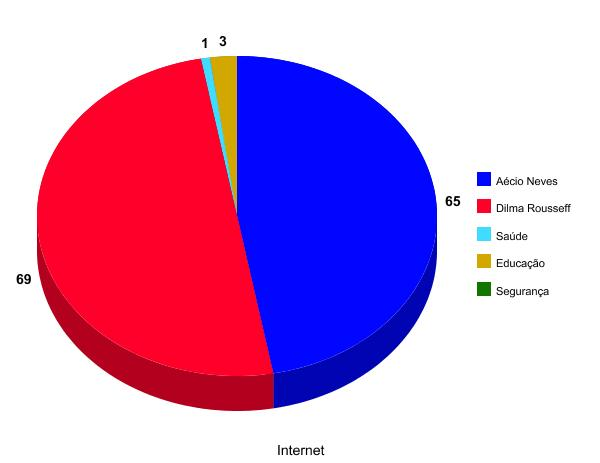
\includegraphics[width=0.6\paperheight]{graph-todos.jpg}
\caption{Comparação da quantidade de notícias envolvendo "Aécio", "Dilma", "Saúde", "Educação" e "Segurança".}
\end{figure}
\end{frame}

%----------------------------------------------------------------------------------------
%	Slide X - Final
%----------------------------------------------------------------------------------------

\begin{frame}
\Huge{\centerline{Obrigado ;)}}
\end{frame}

%----------------------------------------------------------------------------------------

\end{document}